\documentclass{article}
\usepackage{homework}

\usepackage{graphicx}

\begin{document}

\hwtitle{Report for Assignment \# 3}{CS 5500}{Parker Michaelson}

\namesection{Experience}

Preliminary work on the project was started on Wednesday when I interviewed Dr. Sundberg to gather information about function representation within the algorithm.
Dr. Sundberg indicated that I should use a tree similar to an abstract syntax tree to represent a candidate function in a mutable form suitable for use in a genetic algorithm.
This AST structure was used to represent a function in the final version of the assignment, although stored in an array in the style of a binary heap.

Coding work in earnest began early Friday afternoon, with most of the top level code, including the top level of the genetic algorithm itself, authored by Friday night.
Work resumed Saturday morning by beginning work on the histogram representation used as a training goal for the genetic algorithm, the histogram was completed that night.
While a large portion of Sunday afternoon was spent in religious observance, most of Sunday evening and of Sunday night were used in an attempt to complete the project, by working on the function representation itself.
On Monday, I made a review of my earlier practices and implemented an aggressive top-down programming methodology, which delivered me to the Monday night submission version.
In this version of the codebase, a single NULL pointer error outside of the genetic algorithm resulted in the program crashing after completing the algorithm but before writing the image to a file.
On Tuesday, an image was generated using the Monday codebase sans NULL pointer bug, this image is included in the report.       

\namesection{Results}

\begin{figure}[htbp]
        \centering
        \begin{minipage}{.5\textwidth}
                \centering
                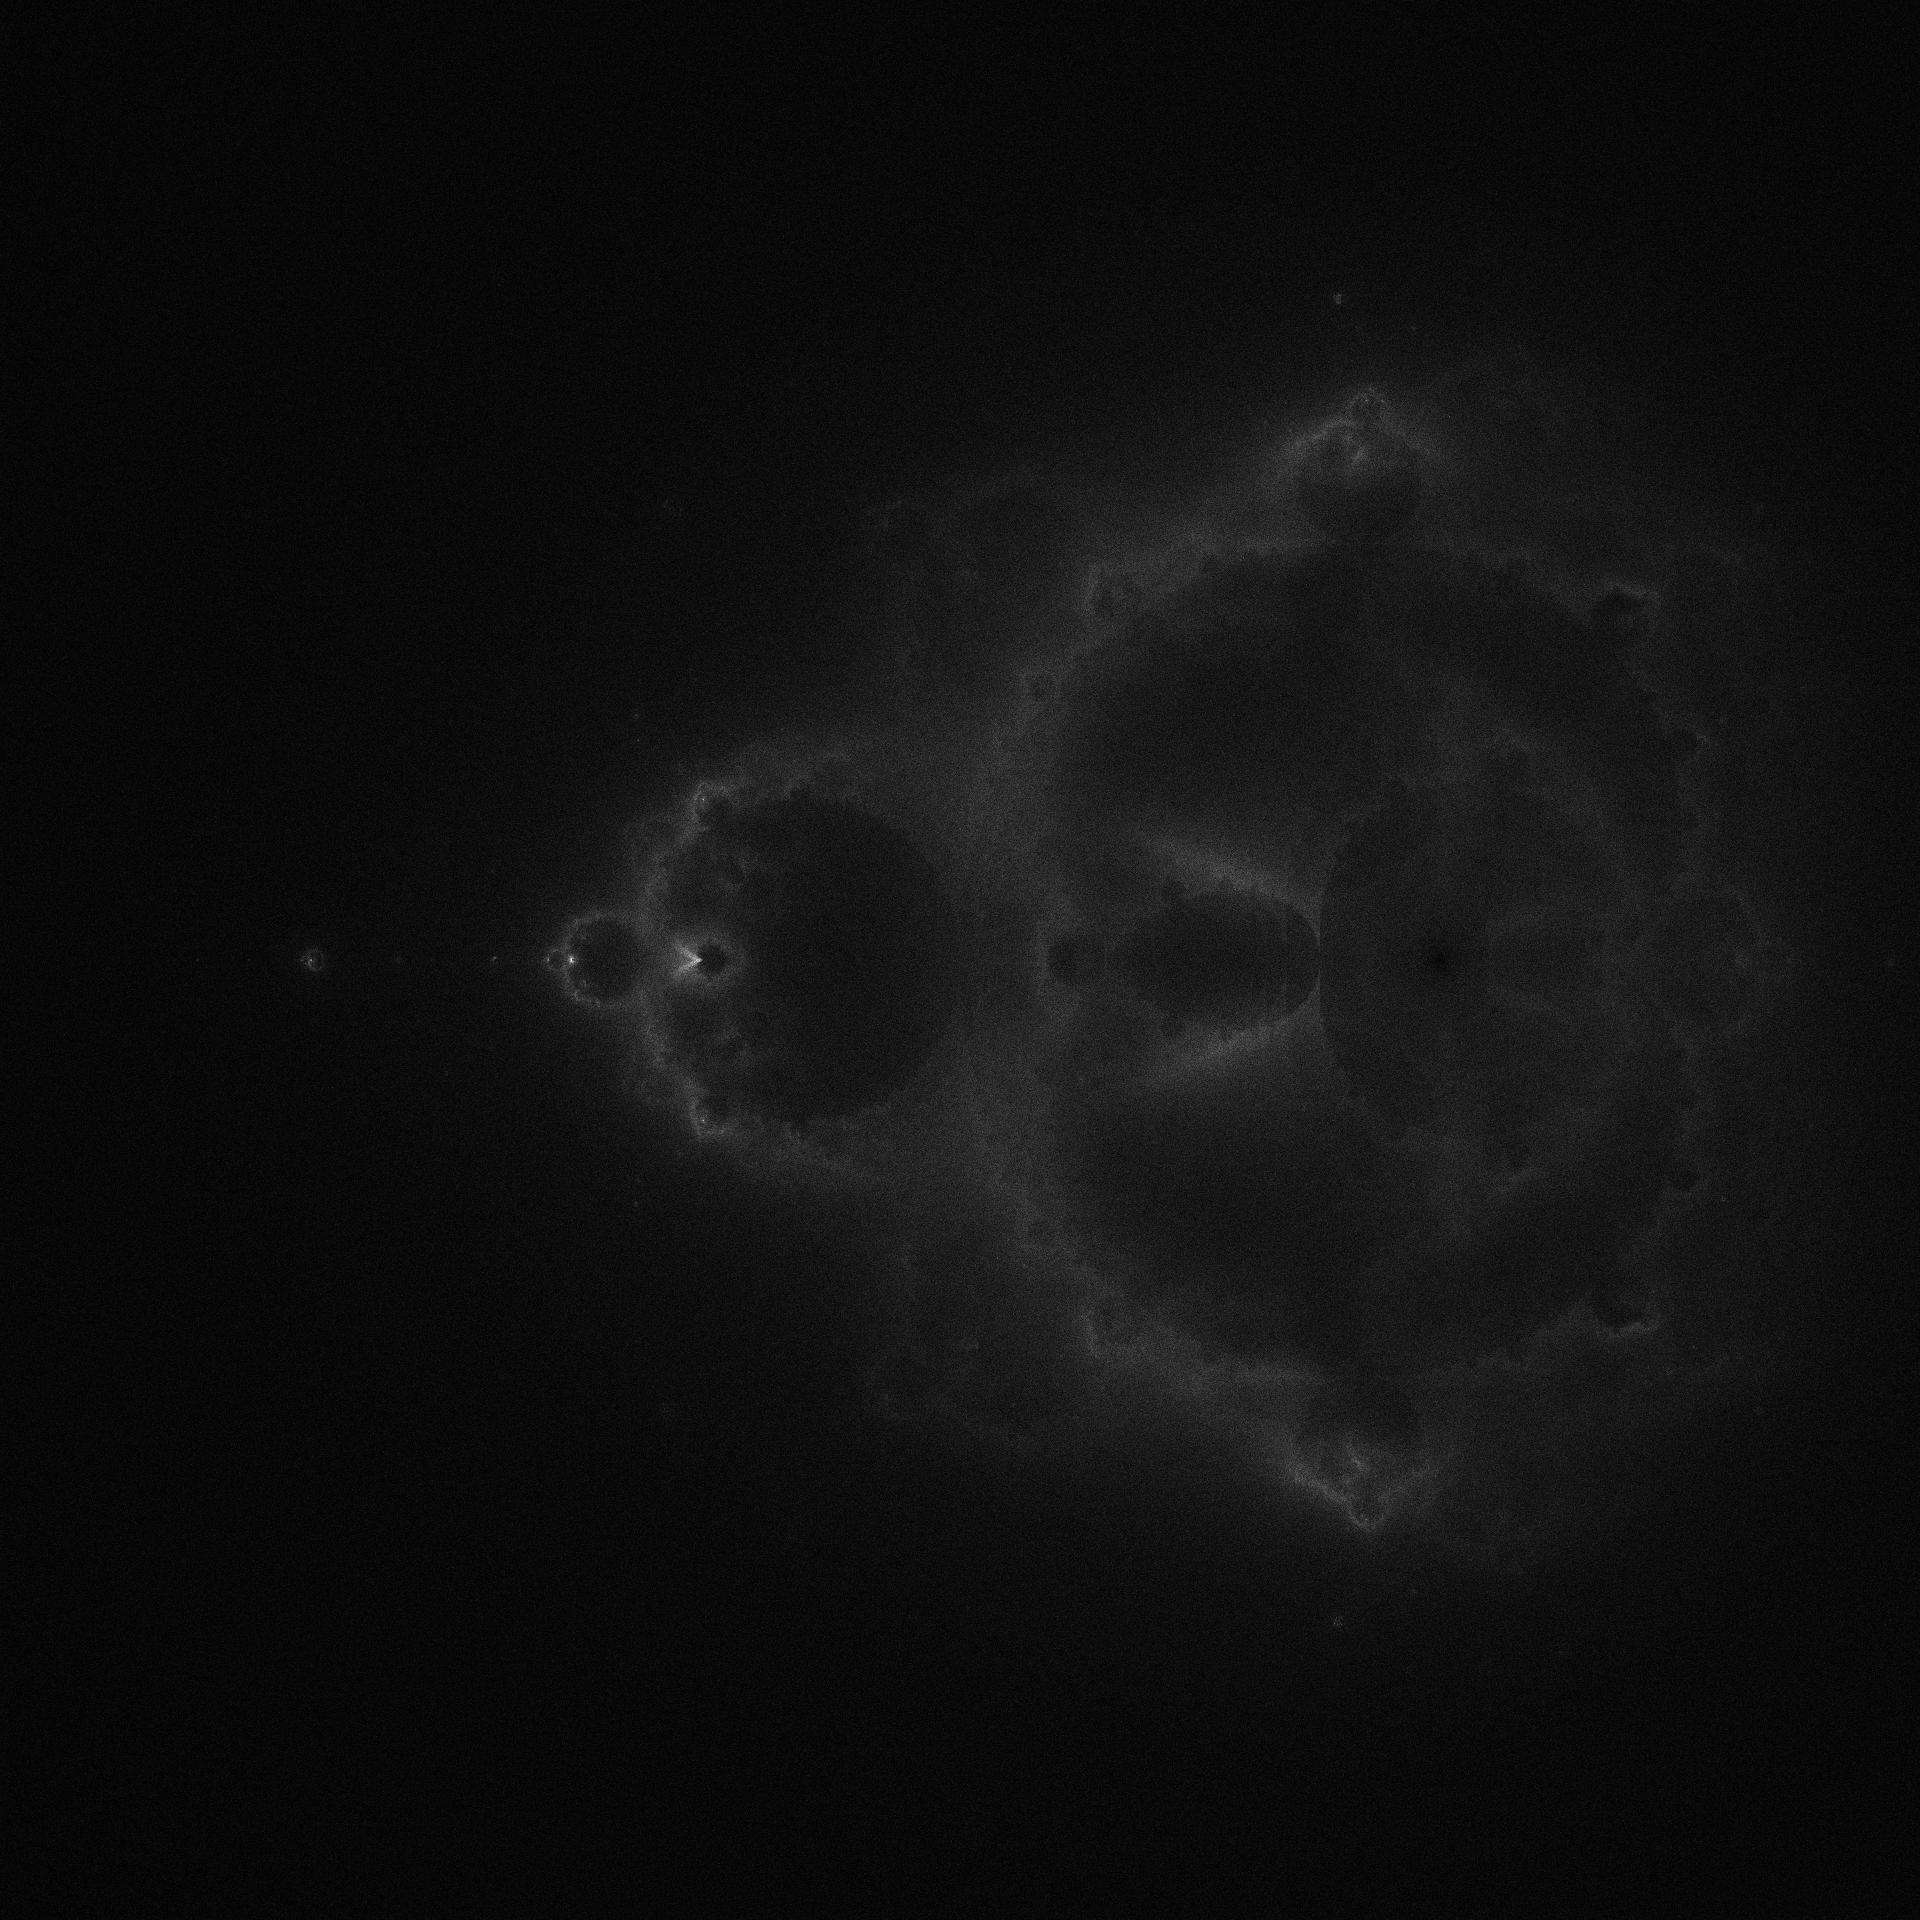
\includegraphics[width=6.6cm]{../master.jpeg}
                \caption{Image used for training the genetic algorithm, from Assignment \# 1}
                \label{fig:fig1}
        \end{minipage}%
        \begin{minipage}{.5\textwidth}
                \centering
                
\includegraphics[width=6.6cm]{../new_result.jpeg}
                \caption{Best result from the final run of the genetic algorithm.}
                \label{fig:fig2}
        \end{minipage}
\end{figure}

It is interesting to note that while the Buddhabrot image itself is mostly black, the genetic algorithm image appears to be completely black. I theorise this to be a result of the maximum complexity of a candidate function, which is composed only of additions, subtractions, multiplications and divisions on X, Y and constants. This results in a ``best solution'' which is simply the presiding color of the Buddhabrot image.

\end{document}
